\documentclass[tikz,border=12pt]{standalone}
\usepackage{amsmath,amssymb}
\usetikzlibrary{calc,arrows.meta}

\begin{document}
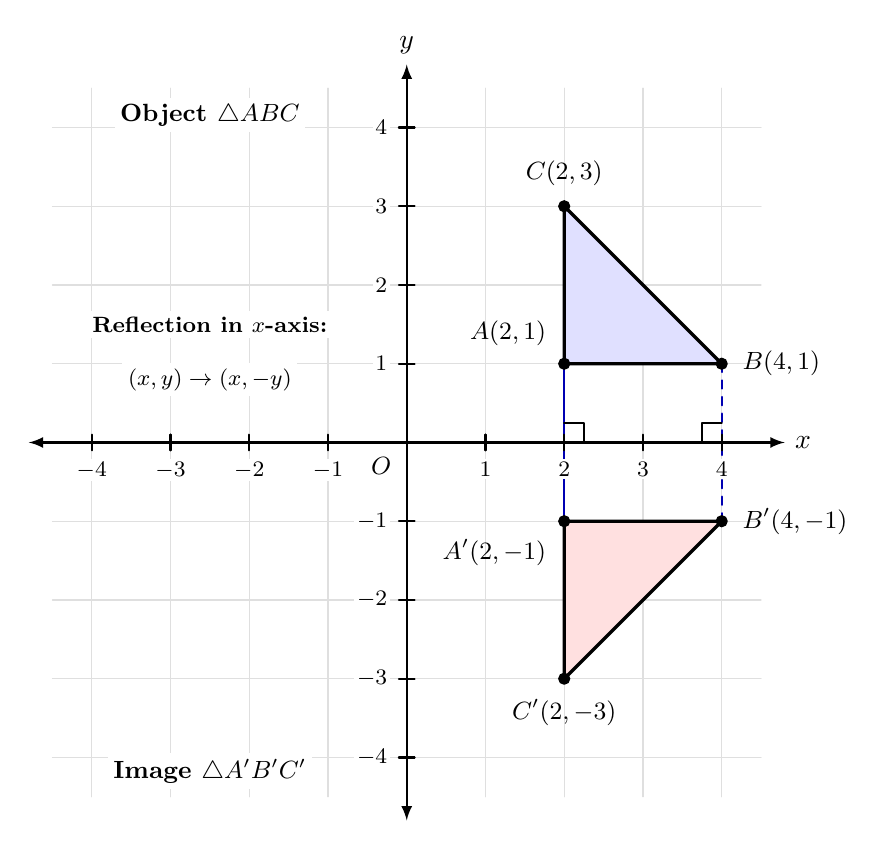
\begin{tikzpicture}[>=latex, line cap=round, line join=round]
  % Grid
  \draw[step=1cm, gray!25, thin] (-4.5, -4.5) grid (4.5, 4.5);

  % Axes
  \draw[thick, <->] (-4.8, 0) -- (4.8, 0) node[right, font=\normalsize] {$x$};
  \draw[thick, <->] (0, -4.8) -- (0, 4.8) node[above, font=\normalsize] {$y$};

  % Origin
  \node[below left=2pt, font=\small] at (0, 0) {$O$};

  % Object triangle ABC (Quadrant I)
  \coordinate (A) at (2, 1);
  \coordinate (B) at (4, 1);
  \coordinate (C) at (2, 3);

  % Dashed reflection projection lines across x-axis
  \draw[thick, dashed, blue!70!black] (A) -- (2, -1);
  \draw[thick, dashed, blue!70!black] (B) -- (4, -1);
  \draw[thick, dashed, blue!70!black] (C) -- (2, -3);

  % Triangles
  \draw[very thick, fill=blue!12] (A) -- (B) -- (C) -- cycle;
  \filldraw[black] (A) circle (2pt) node[above left=3pt, font=\small\bfseries] {$A(2,1)$};
  \filldraw[black] (B) circle (2pt) node[right=4pt, font=\small\bfseries] {$B(4,1)$};
  \filldraw[black] (C) circle (2pt) node[above=4pt, font=\small\bfseries] {$C(2,3)$};

  % Reflected image triangle A'B'C' across x-axis (Quadrant IV)
  \coordinate (A1) at (2, -1);
  \coordinate (B1) at (4, -1);
  \coordinate (C1) at (2, -3);

  \draw[very thick, fill=red!12] (A1) -- (B1) -- (C1) -- cycle;
  \filldraw[black] (A1) circle (2pt) node[below left=3pt, font=\small\bfseries] {$A'(2,-1)$};
  \filldraw[black] (B1) circle (2pt) node[right=4pt, font=\small\bfseries] {$B'(4,-1)$};
  \filldraw[black] (C1) circle (2pt) node[below=4pt, font=\small\bfseries] {$C'(2,-3)$};

  % Right angle markers on mirror line
  \draw[thick] (2, 0.25) -- (2.25, 0.25) -- (2.25, 0);
  \draw[thick] (4, 0.25) -- (3.75, 0.25) -- (3.75, 0);

  % Annotations cleanly positioned in Quadrant II & III
  \node[above=4pt, font=\small\bfseries, fill=white, inner sep=2pt] at (-2.5, 3.8) {Object $\triangle ABC$};
  \node[below=4pt, font=\small\bfseries, fill=white, inner sep=2pt] at (-2.5, -3.8) {Image $\triangle A'B'C'$};
  \node[font=\footnotesize\bfseries, fill=white, inner sep=2pt] at (-2.5, 1.5) {Reflection in $x$-axis:};
  \node[font=\footnotesize, fill=white, inner sep=2pt] at (-2.5, 0.8) {$(x, y) \to (x, -y)$};

  % Integer ticks with opaque backgrounds drawn last so labels never collide
  % with the projection lines passing through them
  \foreach \x in {-4,-3,-2,-1,1,2,3,4} {
    \draw[thick] (\x, 0.1) -- (\x, -0.1);
    \node[below=3pt, font=\footnotesize, fill=white, inner sep=1pt] at (\x, -0.1) {$\x$};
  }
  \foreach \y in {-4,-3,-2,-1,1,2,3,4} {
    \draw[thick] (0.1, \y) -- (-0.1, \y);
    \node[left=3pt, font=\footnotesize, fill=white, inner sep=1pt] at (-0.1, \y) {$\y$};
  }

\end{tikzpicture}
\end{document}
